
\begin{figure}
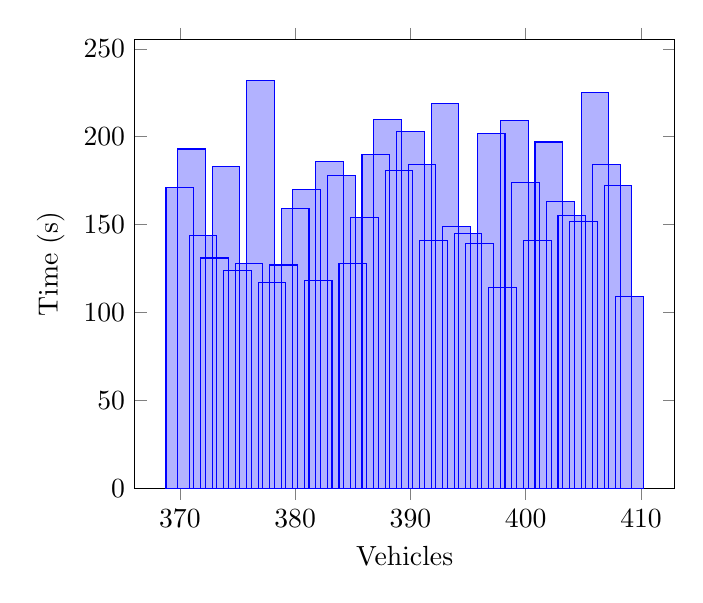
\begin{tikzpicture}
\begin{axis}[
legend style={anchor=west},
xlabel=Vehicles,
ylabel=Time (s),
ymin=0,
ybar,
]
\addplot coordinates {
(407, 184)
(406, 225)
(405, 152)
(403, 163)
(402, 197)
(401, 141)
(400, 174)
(409, 109)
(379, 127)
(378, 117)
(370, 171)
(373, 131)
(375, 124)
(374, 183)
(393, 219)
(392, 141)
(391, 184)
(397, 202)
(396, 139)
(395, 145)
(394, 149)
(398, 114)
(380, 159)
(381, 170)
(382, 118)
(383, 186)
(384, 178)
(385, 128)
(386, 154)
(387, 190)
(388, 210)
(389, 181)
(404, 155)
(408, 172)
(371, 193)
(377, 232)
(376, 128)
(390, 203)
(372, 144)
(399, 209)
};

\end{axis}
\end{tikzpicture}
\label{tik:time:0:56}
\caption{0 percent diving with GSC on route $56$}
\end{figure}
